\input{../YKY-preamble.tex}

\usepackage{color}
\usepackage{mathtools}
\usepackage{hyperref}

% \usepackage[backend=biber,style=numeric]{biblatex}
% \bibliography{../AGI-book}
% \renewcommand*{\bibfont}{\footnotesize}

\usepackage{graphicx} % Allows including images
\usepackage{tikz-cd}
\usepackage{tikz}
\usetikzlibrary{shapes}
\usepackage[export]{adjustbox}% http://ctan.org/pkg/adjustbox
\usepackage{bm}
\usepackage{verbatim} % for comments
\usepackage[most]{tcolorbox}
% \usepackage{newtxtext,newtxmath}	% Times New Roman font

% \numberwithin{equation}{subsection}

\newcommand{\underdash}[1]{%
	\tikz[baseline=(toUnderline.base)]{
		\node[inner sep=1pt,outer sep=10pt] (toUnderline) {#1};
		\draw[dashed] ([yshift=-0pt]toUnderline.south west) -- ([yshift=-0pt]toUnderline.south east);
	}%
}%

\newcommand{\bO}[0]{$\pmb{\bm{\Circle}}$}
\newcommand{\bX}[0]{$\pmb{\bm{\times}}$}

\DeclareSymbolFont{symbolsC}{U}{txsyc}{m}{n}
\DeclareMathSymbol{\strictif}{\mathrel}{symbolsC}{74}

\newcommand{\highlight}[1]{\colorbox{pink}{$\displaystyle #1$}}

\newcommand{\emp}[1]{{\color{violet}\textbf{#1}}}
\newcommand*\confoundFace{$\vcenter{\hbox{\includegraphics[scale=0.2]{../2020/../confounded-face.jpg}}}$}
\newcommand{\underconst}{\includegraphics[scale=0.5]{../2020/UnderConst.png}}
\newcommand{\witness}{\scalebox{0.6}{$\blacksquare$}}
% \newcommand{\Heytingarrow}{\mathrel{-}\mathrel{\triangleright}}
\providecommand\Heytingarrow{\relbar\joinrel\mathrel{\vcenter{\hbox{\scalebox{0.75}{$\rhd$}}}}}

\begin{document}

\title{\bfseries\color{blue}{\Huge AGI standard model}\\ --- trying to establish a consensus}
\author{YKY} % Your name
%\institute[] % Your institution as it will appear on the bottom of every slide, may be shorthand to save space
%{
%Independent researcher, Hong Kong \\ % Your institution for the title page
%\medskip
%\textit{generic.intelligence@gmail.com} % Your email address
%}
\date{\today} % Date, can be changed to a custom date

\maketitle

% \vspace*{0.5cm}
% 多谢 支持 \smiley

\setcounter{section}{-1}
\section{Introduction}

The ``standard model'' is a way of thinking, that may help us better understand the general theory of AGI systems.

The essence of the standard model is just to identify a \textbf{Working Memory} or ``state'' of the AGI system.

One benefit of our theory is that it relates Transformers / BERT / GPT to AGI systems.  These language models are phenomenally intelligent, yet many people criticize them as not ``truly'' intelligent.  The standard model suggests that they are indeed linked to AGI.  There are other benefits.

\section{Reinforcement learning}

This is the simplest form of a \textbf{dynamical system}:
\begin{equation}
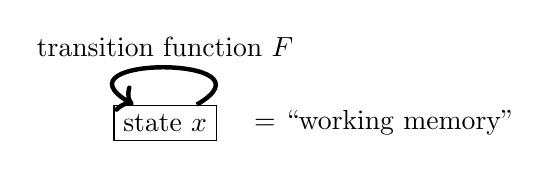
\begin{tikzpicture}[->]
\node[rectangle,draw,label=0:{{$\quad =$} ``working memory"}] (C) {state $x$};
\path (C) edge [out=30,in=150,looseness=4,ultra thick] node [above] {transition function $F$} (C);
\end{tikzpicture}
\end{equation}
When we add an ``action'' or ``control'' variable $u$ to it, it becomes the most basic  \textbf{control system}:
\begin{equation}
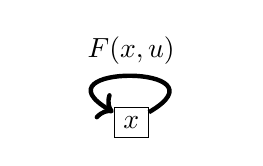
\begin{tikzpicture}[->]
\node[rectangle,draw] (C) {$x$};
\path (C) edge [out=30,in=150,looseness=7,ultra thick] node [above] {$F(x, u)$} (C);
\end{tikzpicture}
\end{equation}
which is the setting for Dynamic Programming or \textbf{Reinforcement Learning}.  The optimal solution for such systems is governed by the \textbf{Hamilton-Jacobi-Bellman equation}.

I call this the ``standard model'' because of the extreme simplicity of this setup, and that I don't know of other alternative models that deviate much from it.

%\section{The standard model in relation to other systems}

Next we look at how the standard model relates to other important aspects of AGI:
\begin{equation}
\vcenter{\hbox{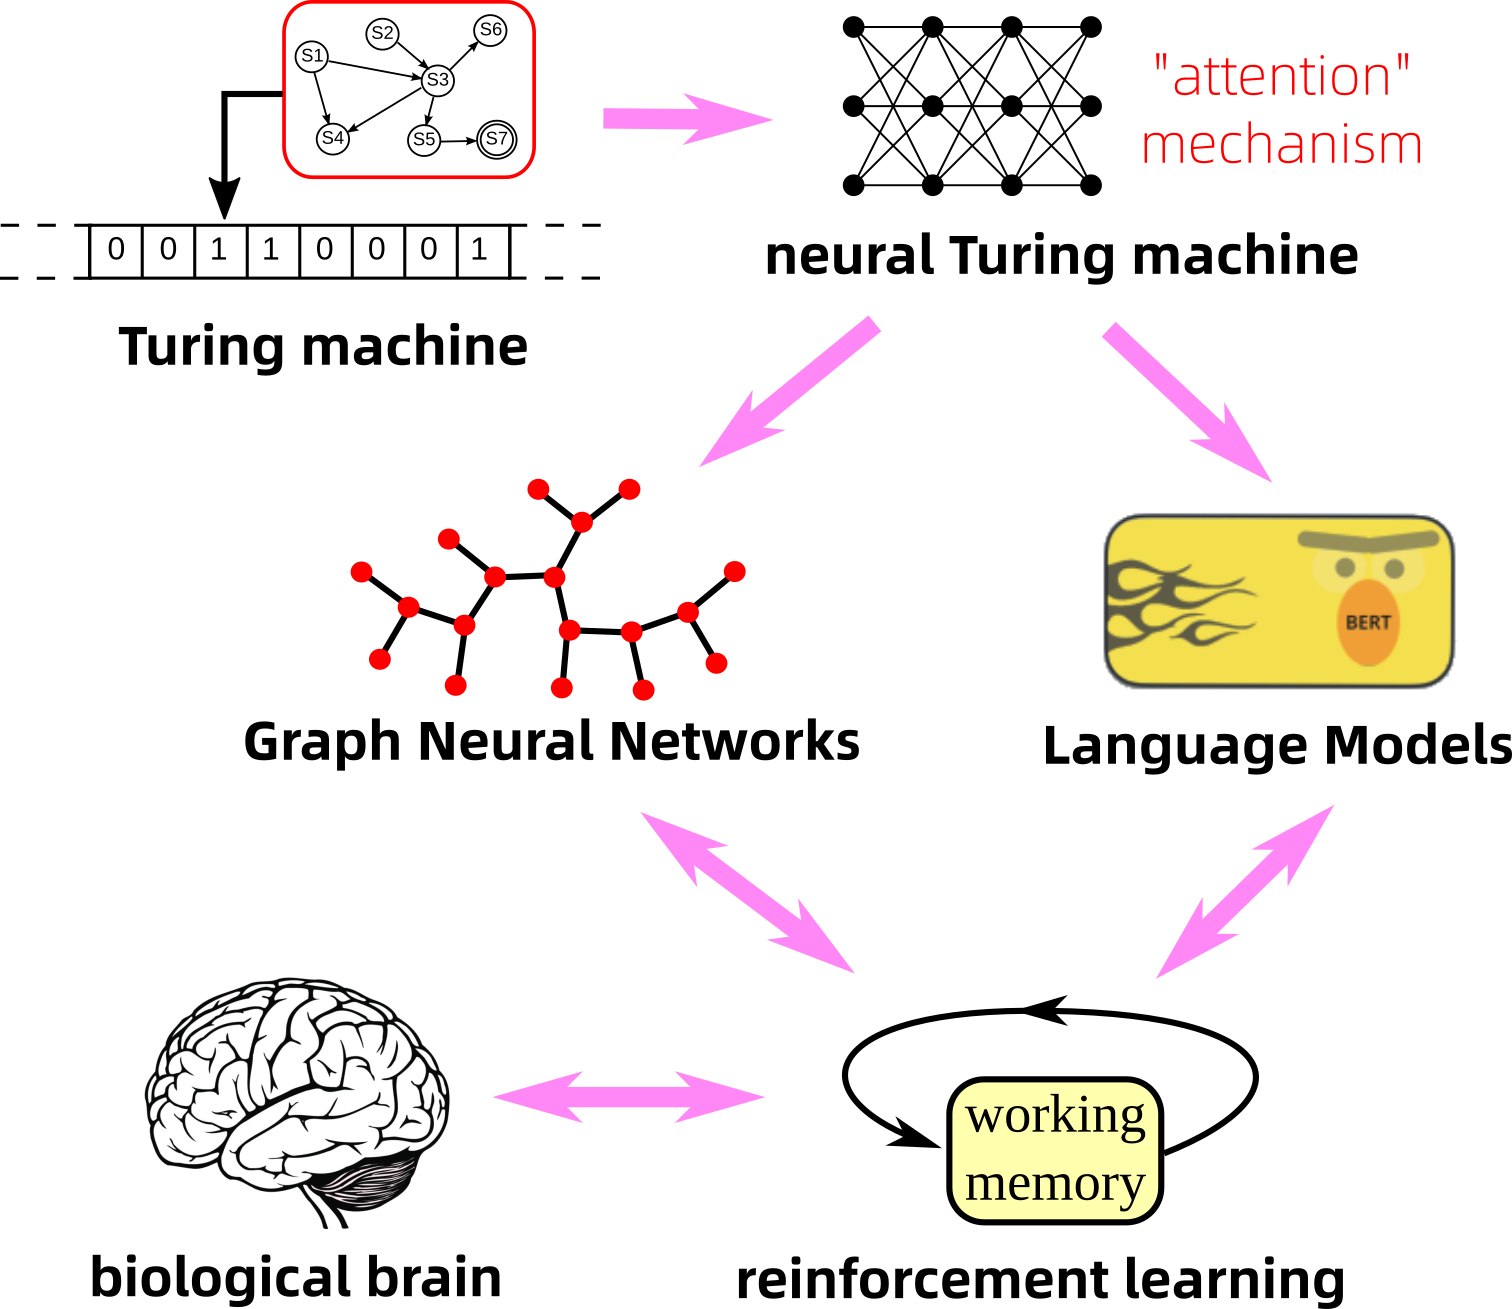
\includegraphics[scale=0.9]{AGI-standard-model.png}}}
\end{equation}

\section{Neural Turing Machine and BERT}

The \textbf{attention mechanism} was first proposed in the ``\textbf{Neural Turing Machine}'' paper by Graves \textit{et al}.

Recall that a Turing machine is a \textbf{Finite State Machine} augmented with a \textbf{Memory Tape}:
\begin{equation}
\vcenter{\hbox{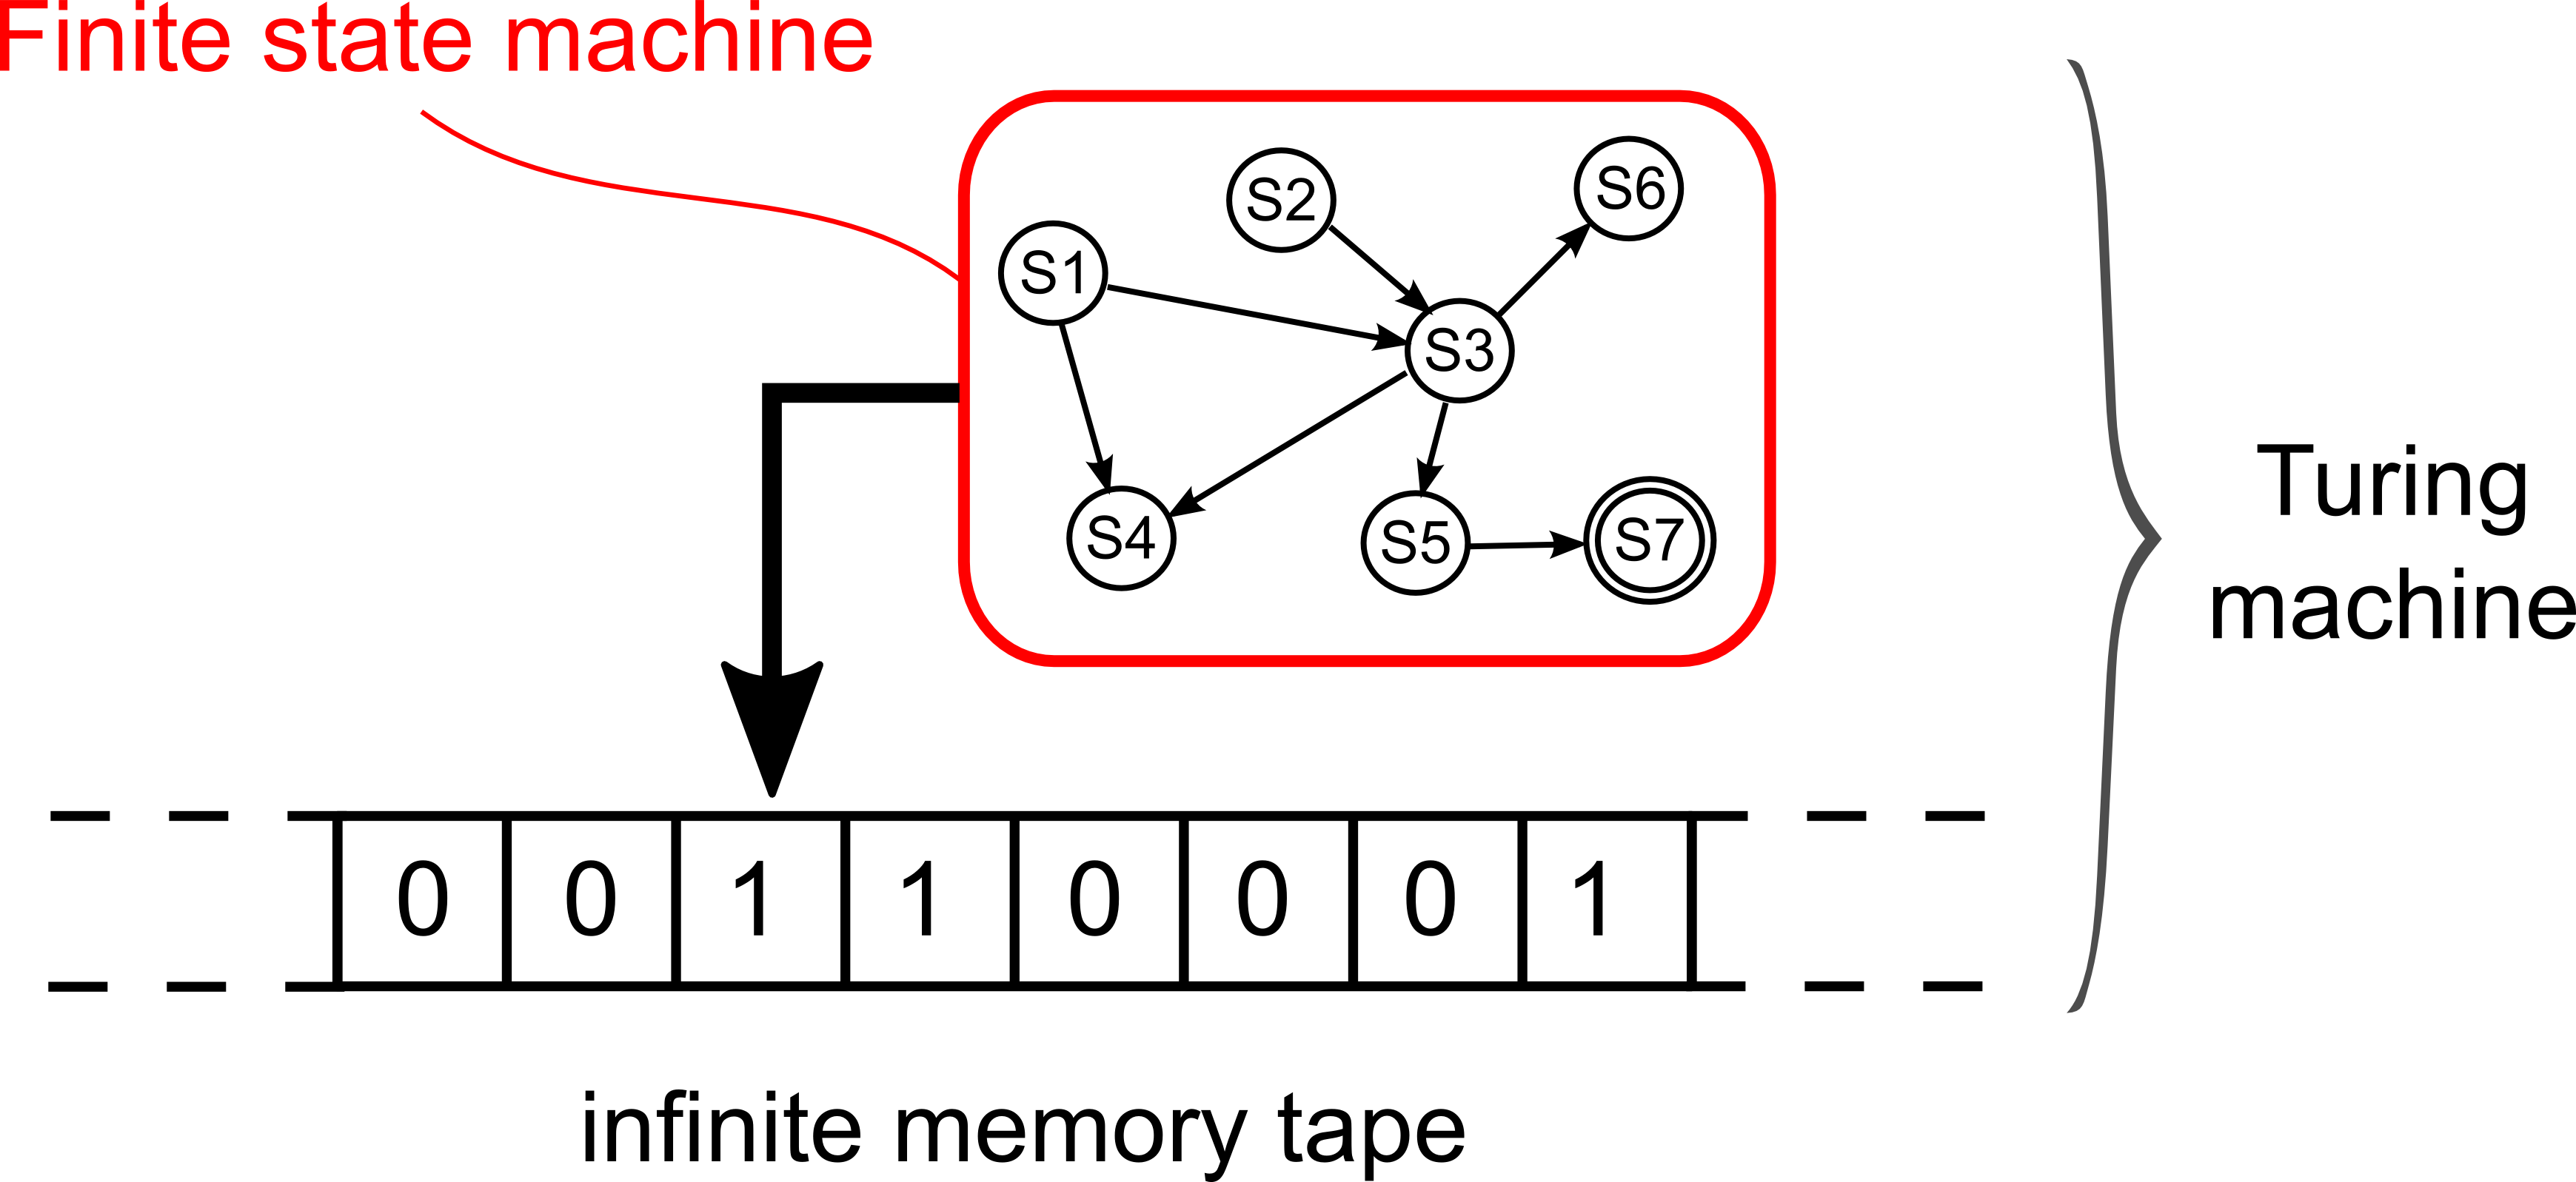
\includegraphics[scale=0.9]{Turing-machine.png}}}
\end{equation}

In Neural Turing Machines, Graves \textit{et al} proposed the attention mechanism for an RNN to read and write from a \textbf{Memory Matrix}, using a content-based addressing method.

The research done by Olah \textit{et al}, in their paper \textit{A Mathematical Framework for Transformer Circuits}, is very helpful towards understanding Transformers and Self-Attention.  The paper is technically quite challenging, but thanks to the guidance of professor Xiao Da from Beijing I was able to understand the main ideas.  Here I offer some pointers to help others understand the paper, without explaining it in full details.

First, it is helpful to recall this diagram describing Self-Attention (ripped from a blog article on the web):
\begin{equation}
\vcenter{\hbox{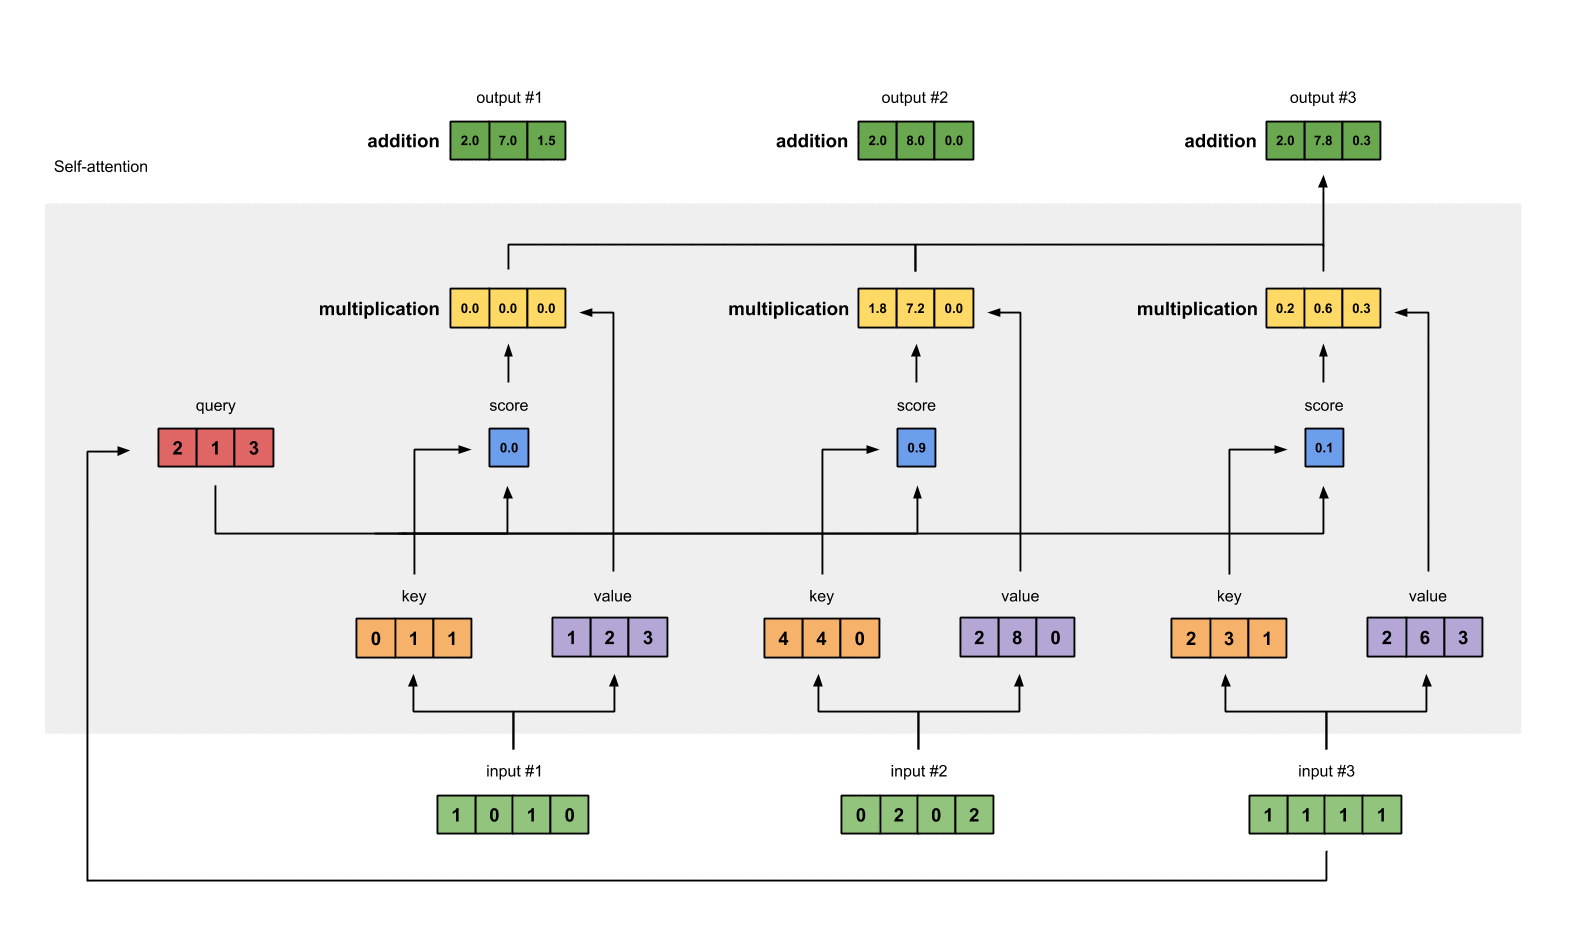
\includegraphics[scale=0.35]{self-attention.png}}}
\end{equation}

The Self Attention $A$ is held constant.

Just as a linear map is defined between two vector spaces:
\begin{equation}
F: U \rightarrow V
\end{equation}
one can define a bi-linear map:
\begin{equation}
\Phi : V \times W \rightarrow U
\end{equation}
that is linear in both its first and second arguments.  The tensor product $\otimes$ is the \textbf{universal} bi-linear map.

The tensor product generalizes to the mathematically important \textbf{monoidal categories}.

Eigen-value plots show that ``copy'' maps are ubiquitous in Transformers.  These may be interpreted as universally-quantified ($\forall$) logic rules.

\section{Relation to the biological brain}

There are two distinct aspects in the brain:
\begin{itemize}
	\item \textbf{Short-term} or Working Memory is the \textbf{electric activation} of neuronal populations.
	\item \textbf{Long-term} memory is stored as \textbf{synaptic strengths}, established by synaptic formation and strengthening.  The transfer from STM to LTM is called \textbf{memory consolidation}.
\end{itemize}

One theory has it that the prefrontal cortex maintains a number of ``thoughts'' with sub-populations or, perhaps, with \textbf{micro-columns}.  These activated sub-populations are in competition with each other, through \textbf{lateral inhibition}.  The thought(s) that win are the thoughts we retain -- they ``make sense''.

\section{Abductive reasoning}

Abductive reasoning is basically just \textbf{bidirectional} inference.

When a system has both forward and backward connections, it forms a loop and its dynamics is likely to produce ``resonance''.  This harks back to the ART (Adaptive Resonance Theory) proposed by Grossberg and Carpenter beginning in the 1980s.

Such resonance behavior can be viewed as the system seeking to minimize an energy, ie, trying to find the ``best explanation'' to a set of facts.  

\section{Dealing with assumptions}

Example of an assumption:  ``If I play move $x$ now, I will checkmate in 3 moves".

Suppose $M, N$ are proofs of $M: \phi \rightarrow \psi$ and $N: \phi$.  Then the proof of $\psi$ would be the application of $M$ to $N$, denoted as $@(M, N)$ or simply $M N$.

The assumption rule (Ax):
\begin{equation}
\Gamma, \phi \vdash \phi \qquad (\mbox{Ax})
\end{equation}
for example can be written as:
\begin{equation}
x : \phi, \; y : \psi \vdash x : \phi \qquad (\mbox{Ax})
\end{equation}
which is why we say that an assumption is a \textbf{$\lambda$-variable}.  

\textbf{Discharging} an assumption (ie, using the $\rightarrow$I rule) results in a $\lambda$-term.

An AGI needs the ability to place an implication $\phi \rightarrow \psi$ into working memory, and to prove it using the ($\rightarrow$ I) rule, ie, by making an assumption.

\begin{tcolorbox}[breakable, parbox=false, fonttitle=\bfseries, title=Tic Tac Toe example]

% \subsection{Tic Tac Toe example}

Assume the current board is
\scalebox{0.5}{
\begin{tabular}{c|c|c}
	    &     & \bO \\ \hline
	\bO & \bX &     \\ \hline
	\bX &     & 
\end{tabular}} and it's \bX's turn to play.

\bX \ can do the ``double fork'' by playing
\scalebox{0.5}{
\begin{tabular}{c|c|c}
		&     & \bO \\ \hline
	\bO & \bX &     \\ \hline
	\bX &     & {\color{red}\bX}
\end{tabular}}.

But how can an AGI know (or prove) this?

If the current board is 
\scalebox{0.5}{
\begin{tabular}{c|c|c}
		&     & \bO \\ \hline
	\bO & \bX &     \\ \hline
	\bX &     & \bX
\end{tabular}}  then a double fork exists.  We need a predicate to detect double forks.

We need to reason that even if \ \bO \ plays the ``blocking'' move
\scalebox{0.5}{
\begin{tabular}{c|c|c}
{\color{red}\bO} &     & \bO \\ \hline
	\bO & \bX &     \\ \hline
	\bX &     & \bX
\end{tabular}}  , \bX \ can still win.

We can easily express the conditions for \bX-can-win, but the difficult part is to make the assumption in {\color{red}red}, in other words:
\begin{equation}
\mbox{{\color{red}red-move}} \rightarrow \mbox{\bX-can-win}
\end{equation}
The difficulty lies in that the LHS is \textbf{not true} under the current facts.  This conditional statement must be proven by, first, assuming the LHS, and then deriving the RHS.  Then the assumption is \textbf{discharged} and the conditional statement is proven, via the ($\rightarrow$ I) rule.

In the old days, in classical AI, assumptions are handled with \textbf{Truth Maintenance Systems} that keep track of inference traces symbolically.  These systems can get quite complicated with the need to track multiple assumptions.  For example, when we plan a bank robbery, we need to consider many possible forking scenarios.  

\end{tcolorbox}

\textbf{Algorithm:}  Put the assumption $A$ in Working Memory.  Make inferences, marking all conclusions with $A \rightarrow *$.  When enough conclusions are obtained, remove the assumption $A$ from Working Memory.

\end{document}
